%{{{ misc
\documentclass[subfigure,epsfig,fleqn,float,numbers=noenddot]{scrartcl}

\usepackage{graphicx}
\usepackage{epstopdf}
\usepackage{caption}
\usepackage{subcaption}
\usepackage{amsmath}

\usepackage{pgfplots}

%Zitieren:
\usepackage[english]{babel}
%\usepackage[german]{babel}
\usepackage{babelbib} % f�r das Erstellen des Bibtex-Literaturverzeichnisses
\usepackage{cite}
%\selectbiblanguage{english}
%\selectbiblanguage{german}

%Peseudocode
\usepackage{algpseudocode}
\usepackage{algorithm}

%Fancy shit
\usepackage{url}

\usepackage[pdftitle={Computer Vision - 2nd Exercise Round},
 						pdfauthor={Matthias Gusenbauer},
						pdfauthor={Robin Mel�n},
						pdfauthor={David Pfahler},
            pdfsubject={Computer Vision},
            pdfborder={0 0 0}]{hyperref}


\usetikzlibrary{plotmarks}
\pgfplotsset{compat=newest} 
\pgfplotsset{plot coordinates/math parser=false}

%%%%%%%%%%%%%%%%%%%%%%%%%%%%%%%%
% Titlepage

\pagestyle{empty}


%set dimensions of columns, gap between columns, and paragraph indent

\setlength{\textheight}{24.7 cm}
\setlength{\columnsep}{1 cm}
\setlength{\textwidth}{16 cm}
%\setlength{\footheight}{0.0 cm}
\setlength{\topmargin}{0.0 cm}
\setlength{\headheight}{0.0 cm}
\setlength{\headsep}{-0.3 cm}
\setlength{\oddsidemargin}{0.0 cm}
\setlength{\parindent}{0 cm}
\setlength{\parskip}{0.5em}
\setlength{\mathindent}{0mm}

% set page counter if document is part of proceedings
\setcounter{page}{1}
\renewcommand{\floatpagefraction}{0.9}
\renewcommand{\textfraction}{0.1}

% Set the Counters like in the exercise sheet
\setcounter{section}{3}
\renewcommand{\thesection}{Assignment \arabic{section}:}
\renewcommand{\thesubsection}{\Alph{subsection}.}

%\renewcommand{\captionlabelfont}{\fontfamily{phv}\fontseries{bx}\fontsize{10}{10pt}\selectfont}
%\renewcommand{\captionfont}{\fontfamily{phv}\fontsize{10}{12pt}\selectfont}
%\setlength{\captionmargin}{0.5 cm}

\makeatletter
\makeatother
\def\RR{\hbox{I\kern-.2em\hbox{R}}}


\begin{document}

%don't want date printed
\date{\today}

%make title bold and 14 pt font (Latex default is non-bold, 16pt) 
\title{~\\
	\fontsize{12}{12pt} \bf Computer Vision 183.585 VU 3.0 4.5 ECTS
  ~\\[0.7cm]
  \fontsize{14}{14pt} \bf 2nd Exercise Round}
  

%for single author 
\author{~\\
  ~\\
  \fontsize{12}{12pt}
  {\bf David Pfahler, Matthias Gusenbauer, Robin Mel�n}\\
  1126287, 1125577, 1029201
  ~\\ ~\\ ~\\
  \normalsize
}

\maketitle
%I don't know why I have to reset thispagestyle, but otherwise get page numbers 
\normalfont
\thispagestyle{empty}

%%%%%%%%%%%%%%%%%%%%%%%%%%%%%%%%%%%%%%%%%%%%%%%%%%%%%%%%%%%%%%%%%%%%%%%%%%%%%%%%
% CONTENT

\section{Image Stitching}
\label{sec:1}

\subsection{SIFT Interest Point Detection}
\label{sec:A}

\subsection{Interest Point Matching and Image Registration}
\label{sec:B}

\subsection{Image Stitching}
\label{sec:C}

\section{Scene Recognition with Bag of Visual Words}
\label{sec:2}

In this assignment we want to classify images into scene categories like bedroom, kitchen etc. 
We use the standard bag of visual words model to achieve this task. Subsection~\ref{sec:methodology} presents the implementation of the category recognition and Subsection~\ref{sec:results} presents our results.

\subsection{Methodology}
\label{sec:methodology}

First the test- and the training-set gets loaded and for every image its category is saved. The next step is to build a vocabulary
of visual words. We will form this vocabulary by sampling many local features from our training set and then clustering them with K-means. The number of K-means clusters \texttt{num\_clusters} is the size of our vocabulary. We used 50 clusters which means that the 128 dimensional SIFT feature space is partitioned into 50 regions.\\
Every time a new SIFT feature gets observed, the cluster it belongs to can easily get figured out by getting the nearest centroid of our original clusters. Those clusters are our visual word vocabulary.\\
To extract these SIFT features from the images in the training set to collect them for k-means clustering, 100 SIFT features get extracted from every image. These features get added to the feature space which is $128 \times \mbox{size of training set}*\mbox{number of features per image}$. In out example the training set contains 800 images and the number of features per image is also 100, that means the feature space is $128 \times 80000$ big. After that the 50 clusters get determined and stored in a matrix.\\
The next step is to build a feature representation for every image in the training set that can be used for the classification of new images later on. An image is represented by the normalized histogram of visual words, which means that all SIFT features of an image are assigned to visual words and the number of occurrences of every word is counted. Therefor we have to get the SIFT features for every image from the training set again, but this time it gets sampled more densely than before. We used a step size of 2. Then we determine the nearest clusters of the sampled SIFT-features and count the number of occurrences. This histogram represents the bag of words for this image.\\
The last step is to classify all the images of the test set to investigate the classification power of the bag of visual words model for our classification task. This is obviously quite similar to the previous step. (Get SIFT features densely sampled (step size is 2) and count number of nearest clusters to this features as bag of words) But this time the visual word histogramm of an image is used for actual classifying it by means with the nearest neighbor method (we used a k of 3) with the previously learned training features and class labels. The result is stored in a confusion matrix. (See Figure~\ref{fig:conf_matrix_test})

\subsection{Results}
\label{sec:results}

\begin{figure}
        \centering
        \begin{subfigure}[b]{0.3\textwidth}
                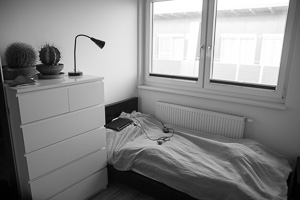
\includegraphics[width=\textwidth]{img/own/bedroom}
                \caption{Bedroom}
                \label{fig:bedroom}
        \end{subfigure}%
        ~ %add desired spacing between images, e. g. ~, \quad, \qquad, \hfill etc.
          %(or a blank line to force the subfigure onto a new line)
        \begin{subfigure}[b]{0.3\textwidth}
                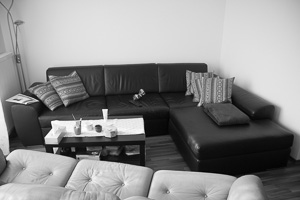
\includegraphics[width=\textwidth]{img/own/livingroom}
                \caption{Livingroom}
                \label{fig:livingroom}
        \end{subfigure}
        ~ %add desired spacing between images, e. g. ~, \quad, \qquad, \hfill etc.
          %(or a blank line to force the subfigure onto a new line)
        \begin{subfigure}[b]{0.3\textwidth}
                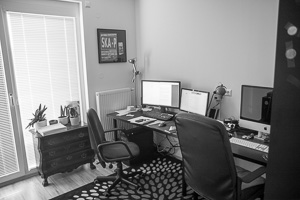
\includegraphics[width=\textwidth]{img/own/office}
                \caption{Office}
                \label{fig:office}
        \end{subfigure}
				
				\begin{subfigure}[b]{0.3\textwidth}
                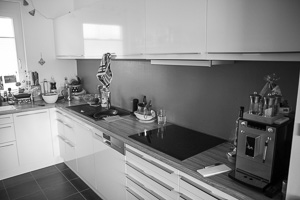
\includegraphics[width=\textwidth]{img/own/kitchen}
                \caption{Kitchen}
                \label{fig:kitchen}
        \end{subfigure}
				~
				\begin{subfigure}[b]{0.3\textwidth}
                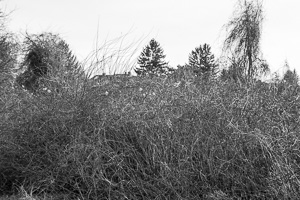
\includegraphics[width=\textwidth]{img/own/forest}
                \caption{Forest}
                \label{fig:forest}
        \end{subfigure}
        \caption{Own scene pictures}\label{fig:ownimages}
\end{figure}

\begin{figure}
		\centering
		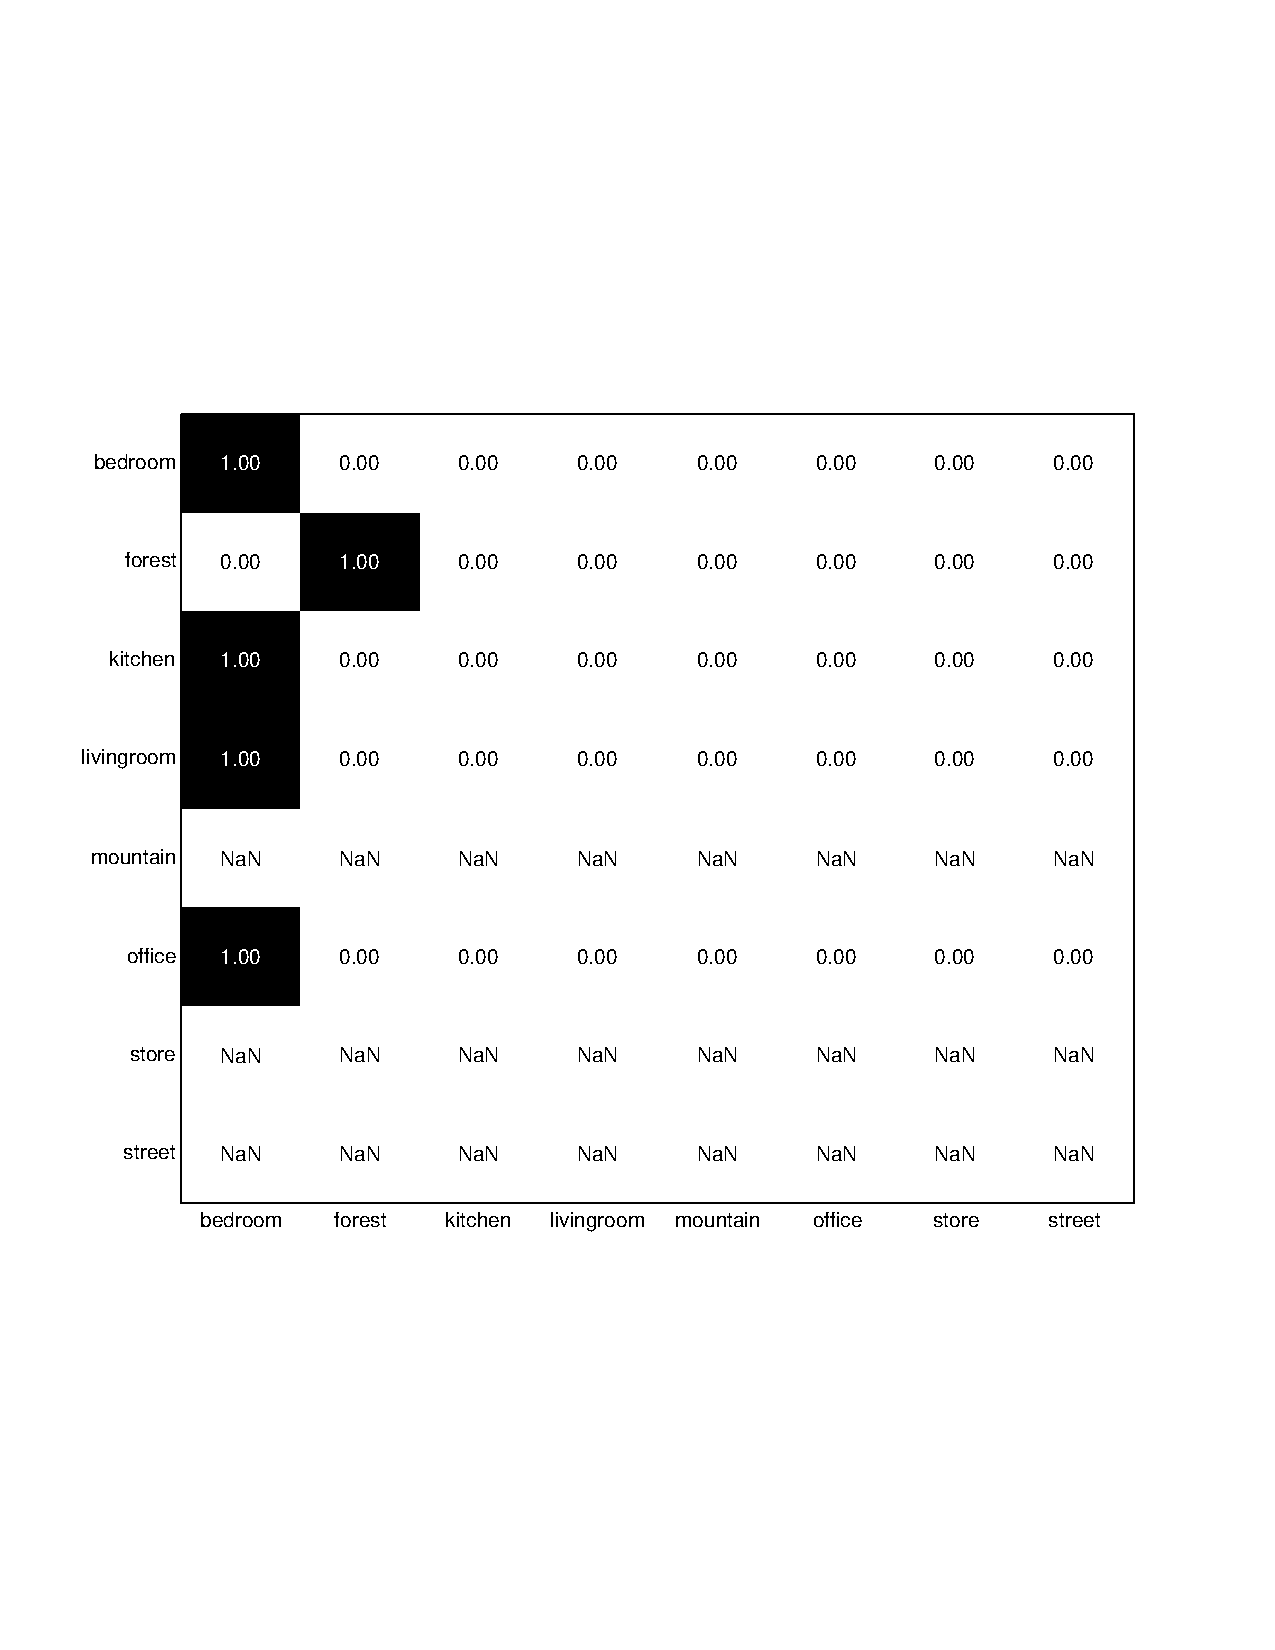
\includegraphics[width=\textwidth]{img/conf_matrix_own.pdf}
		\caption{Conf Matrix Own}
		\label{fig:conf_matrix_own}
\end{figure}
\begin{figure}
		\centering
		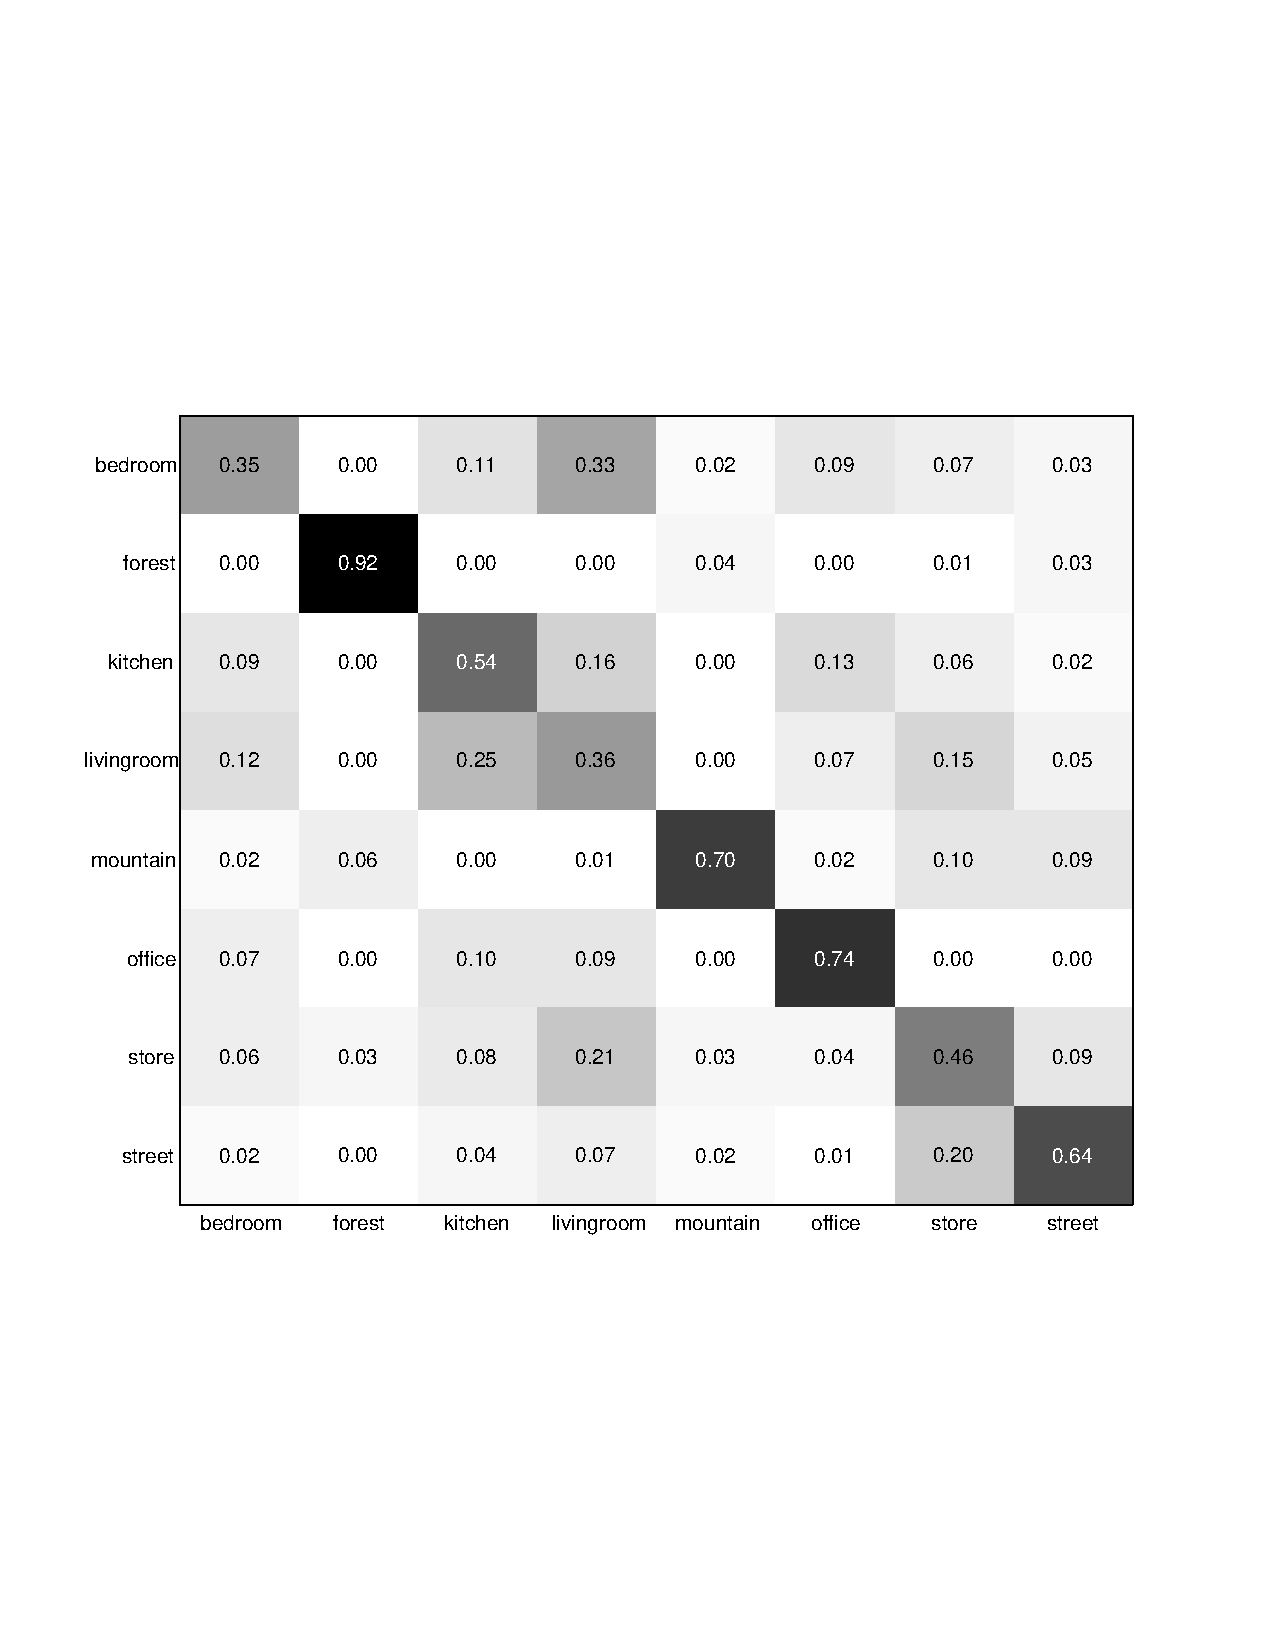
\includegraphics[width=\textwidth]{img/conf_matrix_test.pdf}
		\caption{Conf Matrix Test}
		\label{fig:conf_matrix_test}
\end{figure}

\end{document}

% vim:foldmethod=marker
